\chapter{Algoritmos}
\label{ch::capitulo3}

\section{Introducción}

En este capítulo, presentamos dos algoritmos cuyo objetivo es determinar la equivalencia entre trenzas en el contexto de la teoría de grupos de trenzas. La equivalencia de trenzas es un problema fundamental en este campo, ya que una trenza puede representarse de múltiples formas sin alterar su estructura esencial. Para abordar este problema de forma sistemática, introducimos dos conceptos clave: la \textit{trenza pura} y la \textit{forma normal} de una trenza. Ambos conceptos son cruciales para simplificar la representación de trenzas y permitir su comparación.

\subsection{Trenza pura}

Una \textbf{trenza pura} (\textit{pure braid}) es una trenza en la que cada hebra termina en la misma posición en la que comenzó. En otras palabras, no hay desplazamiento entre las hebras; cada una conserva su identidad al inicio y al final de la trenza. En términos geométricos, esto significa que las marcas o burbujas de color al comienzo y al final de la trenza permanecen alineadas, proporcionando una referencia clara y directa de cada hebra desde el inicio hasta el final. Esta propiedad es valiosa, pues simplifica el análisis de equivalencia al eliminar la complejidad añadida de los desplazamientos de hebras.

\begin{figure}[h!]
    \centering
    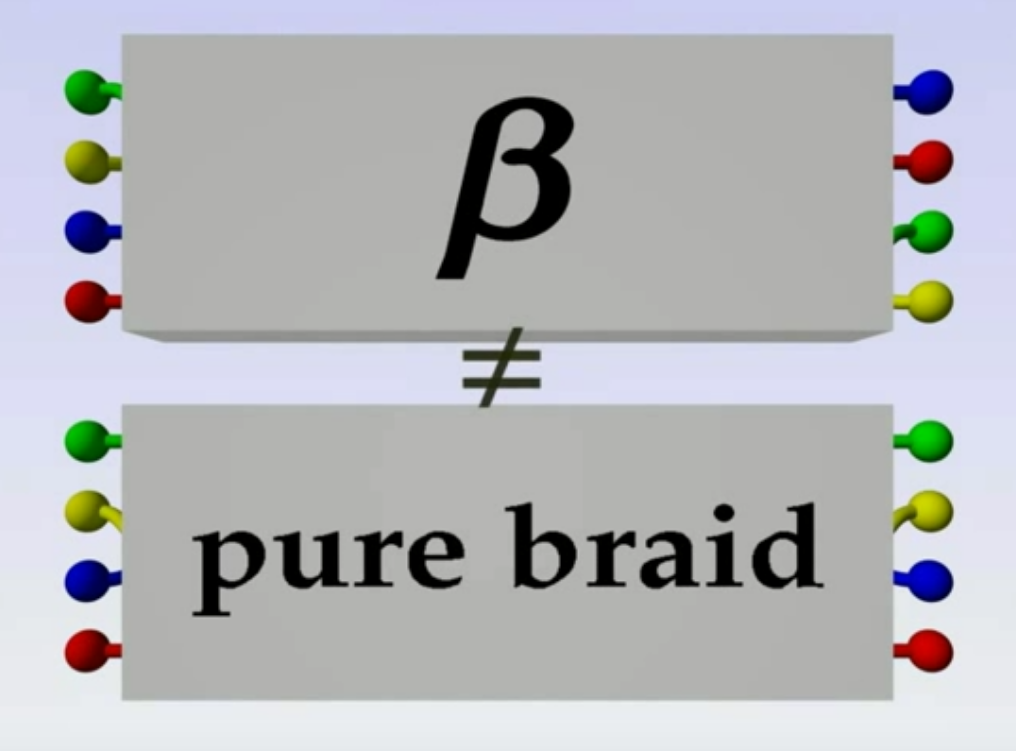
\includegraphics[width=0.5\textwidth]{figures/chapters/3_algoritmos/pure_braid.png}
    \caption{Ejemplo de trenza $\beta$ que no es una trenza pura, ya que los puntos de inicio y fin de algunas hebras no coinciden. Fuente: \cite{esterdalvitBraidsChapter22013}}
\end{figure}

La noción de trenza pura es relevante en el contexto de los algoritmos de comparación, ya que facilita la identificación de configuraciones equivalentes al permitir que cada hebra se rastree fácilmente. Trabajar con trenzas puras es análogo a trabajar con permutaciones en las que cada elemento mantiene su posición, proporcionando una estructura que es más sencilla de manejar y analizar.

\subsection{Forma normal de una trenza}

La \textbf{forma normal} de una trenza es una representación simplificada y única de la trenza, obtenida mediante la reorganización sistemática de sus cruces. El objetivo de la forma normal es reducir la trenza a una expresión estandarizada, eliminando redundancias y ambigüedades en la representación. Si dos trenzas son equivalentes, entonces deben tener la misma forma normal; si sus formas normales difieren, las trenzas representan configuraciones distintas.

\begin{figure}[h!]
    \centering
    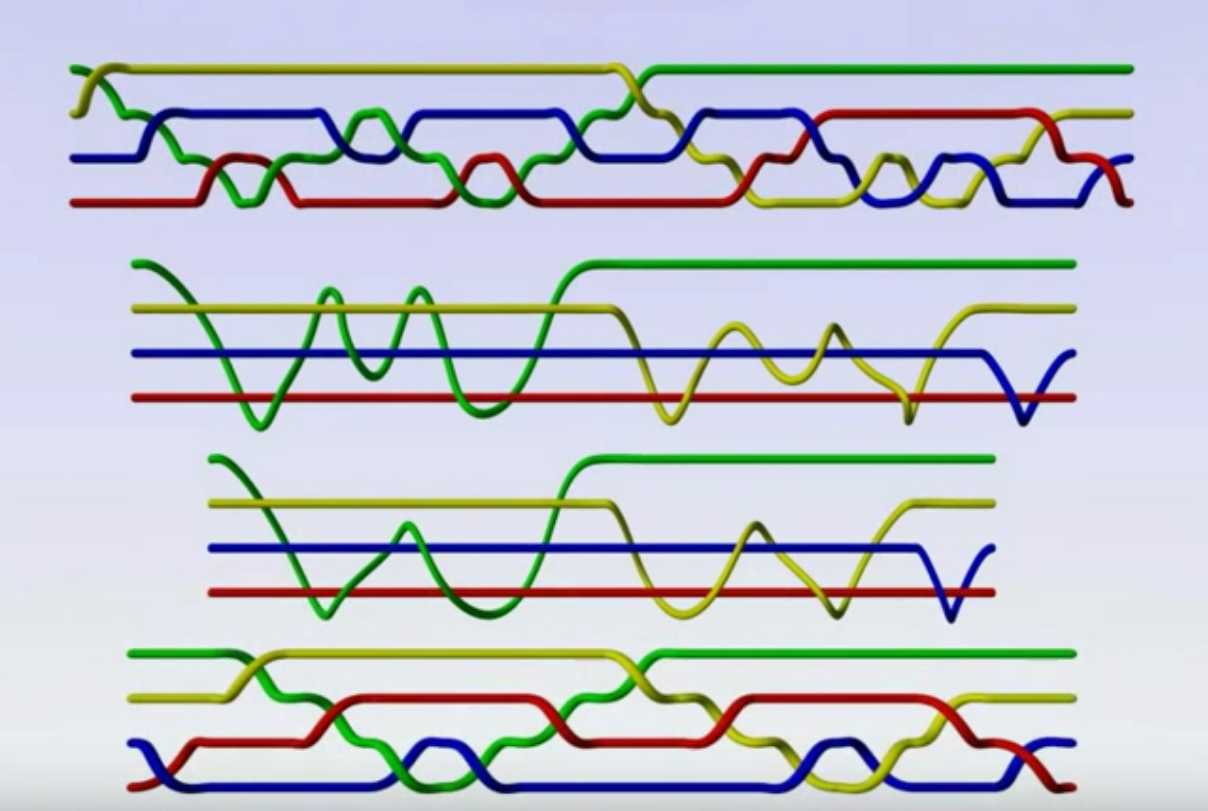
\includegraphics[width=0.4\textwidth]{figures/chapters/3_algoritmos/ejemplos_trenzas_de_una_clase.png}
    \caption{Ejemplo de trenzas pertenecientes a una misma clase. Fuente: \cite{esterdalvitBraidsChapter22013}}
\end{figure}

\begin{figure}[h!]
    \centering
    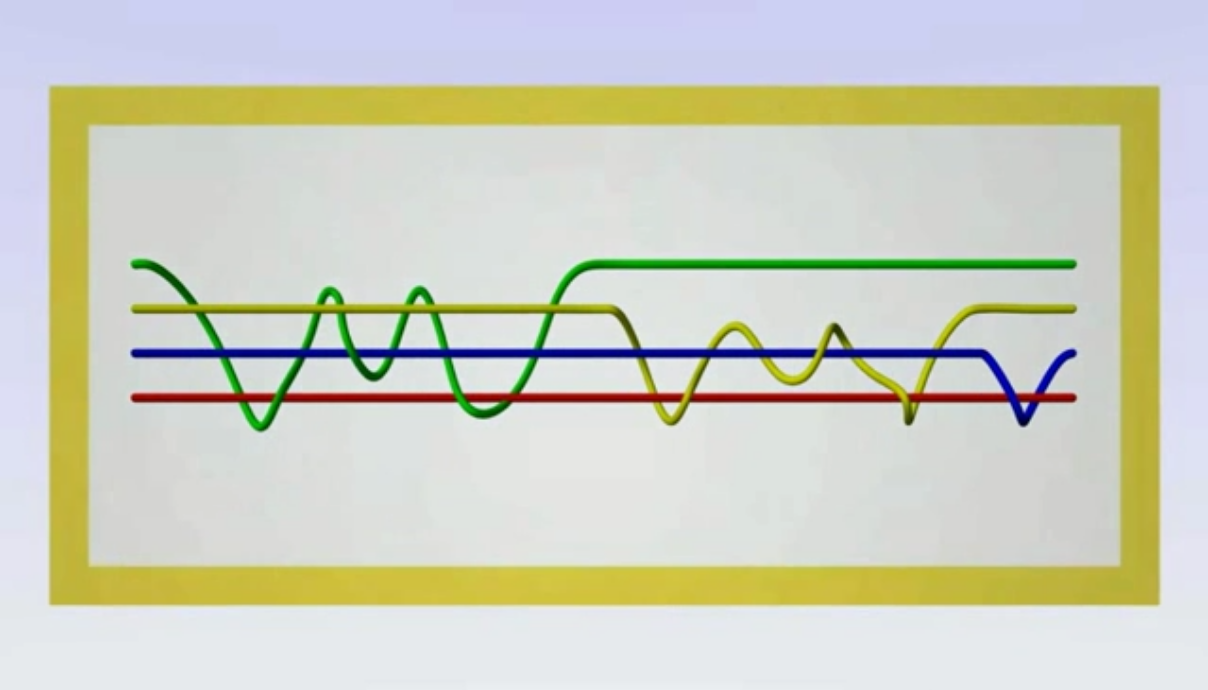
\includegraphics[width=0.5\textwidth]{figures/chapters/3_algoritmos/trenza_normal.png}
    \caption{Trenza normal de la clase anterior. Fuente: \cite{esterdalvitBraidsChapter22013}}
\end{figure}


\newpage

\subsection{Objetivo de los algoritmos}

El propósito de los algoritmos presentados en este capítulo es \textbf{transformar una trenza dada en su forma normal}. Esto permite una comparación directa entre trenzas, eliminando ambigüedades causadas por distintas representaciones de una misma configuración.

Estos algoritmos se basan en reglas de simplificación y conmutación propias del grupo de trenzas. Aplicadas de manera sistemática, estas reglas permiten reducir cada trenza a su forma normal, lo que facilita su comparación con otras trenzas. En el caso de las trenzas puras, esta simplificación es aún más directa, ya que no existen desplazamientos de hebras.

En resumen, este capítulo proporciona herramientas prácticas para determinar la equivalencia de trenzas mediante su transformación a la forma normal, simplificando el proceso de comparación y revelando la estructura esencial de cada trenza dentro del grupo.

\newpage

\section{Braid Combing de Artin}

Para transformar cualquier trenza en su forma normal, Artin introdujo un algoritmo conocido como el \textbf{peinado de trenzas}. Este método organiza la trenza en bloques secuenciales, facilitando el análisis y la comparación. La idea central es ir «peinando» cada hebra de la trenza para simplificar su estructura sin modificar su equivalencia en el grupo de trenzas. A continuación, se describe el proceso general del peinado de Artin, sin detalles específicos sobre cada hebra o bloque.

\subsection{Descripción del algoritmo}

\begin{enumerate}
    \item \textbf{Inicialización}: Se comienza copiando la trenza original y transformando la última hebra en una hebra trivial (sin cruces). Esta trenza modificada se compone con su inversa para crear la trenza identidad, lo que garantiza que no se altera la configuración original. Este primer paso establece el bloque inicial, en el cual todas las hebras son rectas excepto la primera hebra a «peinar».

    \item \textbf{Peinado de cada hebra}: En cada paso, se toma la hebra superior del bloque actual y se deforma para llevarla a su posición final. Esto se realiza haciendo que la hebra pase por detrás o por delante de las otras hebras, siguiendo un recorrido que la sitúa en su posición «peinada» sin cruces innecesarios.

    \item \textbf{Formación de bloques sucesivos}: Para peinar las siguientes hebras, el proceso se repite en bloques sucesivos. En cada bloque, se convierte temporalmente la hebra que se está peinando en una hebra trivial. Luego, esta trenza se compone con su inversa para mantener la identidad, y el bloque resultante se reorganiza para que las hebras se enlacen solo con las que le siguen en el orden, simplificando la estructura general del bloque.

    \item \textbf{Finalización y evaluación de trivialidad}: Una vez peinadas todas las hebras, la trenza se encuentra en su forma normal. Artin demostró que una \textbf{trenza es trivial} si y solo si, al «peinar» la trenza, cada bloque de la trenza resultante es trivial, es decir, no contiene cruces. En esta forma normal, una trenza trivial puede representarse sin cruces, mostrando su equivalencia a la trenza vacía. Este criterio es fundamental para determinar si una trenza es trivial.
\end{enumerate}

\subsection{Limitaciones del algoritmo de Braid Combing}

Aunque el peinado de trenzas de Artin es efectivo para transformar una trenza en su forma normal, tiene una complejidad computacional alta. Cada paso del peinado involucra múltiples operaciones que aumentan exponencialmente con el número de cruces en la trenza. Este crecimiento rápido en el tiempo de ejecución hace que el algoritmo sea ineficiente para trenzas complejas o de gran tamaño.

Artin, consciente de esta limitación, buscó alternativas más rápidas, pues el peinado puede volverse impráctico incluso para una computadora al aumentar ligeramente el tamaño de la entrada.

\subsection{Diagrama de flujo de Braid Combing}

La Figura \ref{fig:diagrama_peinado} muestra el diagrama de flujo del algoritmo de peinado de Artin. En cada paso, el algoritmo verifica si el bloque actual es trivial; si lo es, continúa con el siguiente. Si no lo es y no quedan más bloques, concluye que la trenza no es trivial.

\begin{figure}[h!]
    \centering
    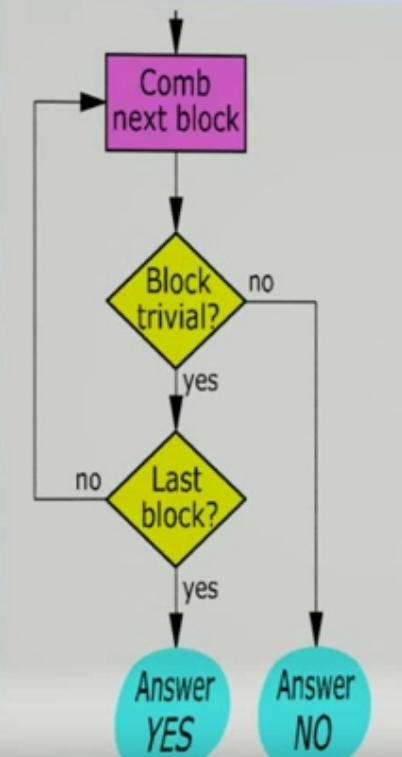
\includegraphics[width=0.4\textwidth]{figures/chapters/3_algoritmos/combing_algorithm.png}
    \caption{Diagrama de flujo del algoritmo de Braid Combing de Artin. Fuente: \cite{esterdalvitBraidsChapter22013}}
    \label{fig:diagrama_peinado}
\end{figure}

\newpage

\section{Reducción de manejadores (Handle Reduction)}

Uno de los algoritmos más rápidos para transformar trenzas en su forma normal fue propuesto por el matemático francés Patrick Dehornoy. Este método, conocido como \textbf{reducción de manejadores}, se basa en identificar y manipular ciertas configuraciones dentro de la trenza, llamadas \textit{manejadores}.

\subsection{Definición y reducción de manejadores}

Un \textbf{manejador} es una configuración en una trenza en la que una hebra pasa dos veces consecutivas por delante (o por detrás) de una hebra vecina, formando un «bucle». Esta estructura permite simplificar el diagrama mediante un proceso llamado \textit{reducción de manejadores}, en el cual el bucle se desplaza hacia un lado, eliminando el manejador sin cambiar la estructura esencial de la trenza.

La Figura \ref{fig:handle_state_1} muestra un ejemplo de un manejador, mientras que la Figura \ref{fig:handle_state_2} ilustra el resultado después de reducir ese manejador. Este proceso de reducción facilita la simplificación de la trenza, sin alterar su configuración fundamental en el grupo de trenzas.

\begin{figure}[h!]
    \centering
    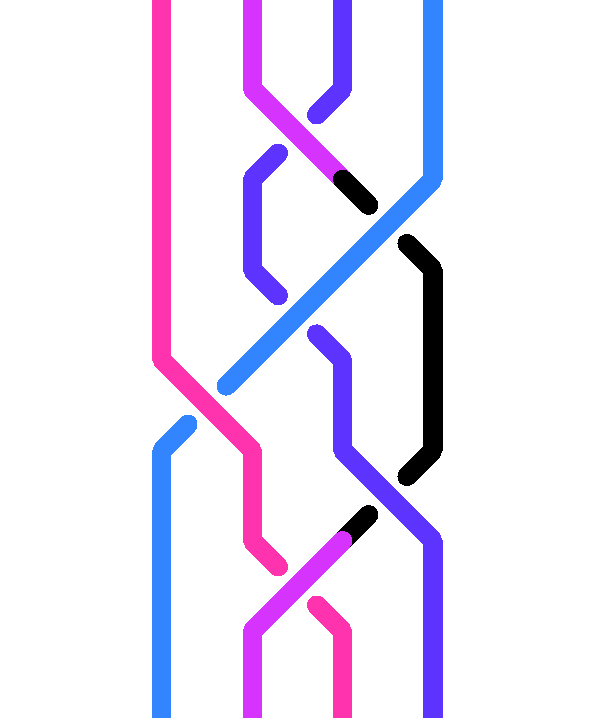
\includegraphics[width=0.2\textwidth]{figures/chapters/3_algoritmos/handle_state_1.png}
    \caption{Ejemplo de un manejador. Fuente: \cite{noauthor_braids_nodate}}
    \label{fig:handle_state_1}
\end{figure}

\begin{figure}[h!]
    \centering
    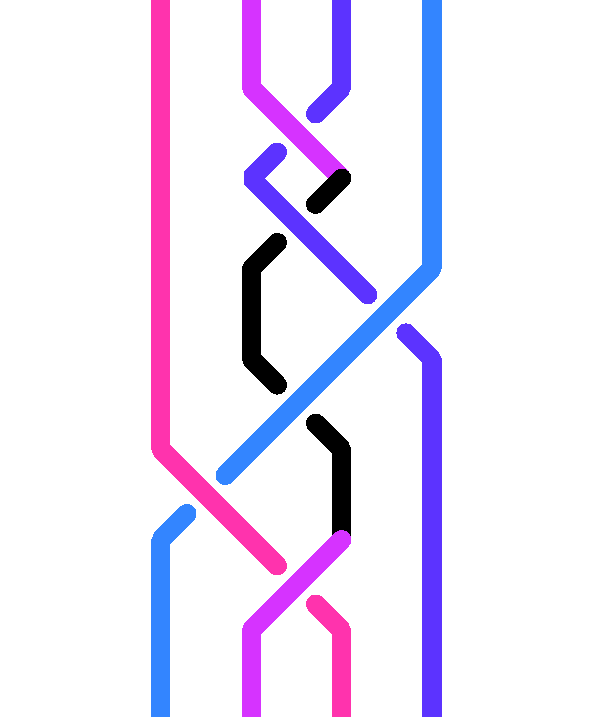
\includegraphics[width=0.2\textwidth]{figures/chapters/3_algoritmos/handle_state_2.png}
    \caption{Ejemplo del resultado tras la reducción de un manejador. Fuente: \cite{noauthor_braids_nodate}}
    \label{fig:handle_state_2}
\end{figure}

\subsection{Algoritmo de reducción de manejadores}

El objetivo del algoritmo es eliminar todos los manejadores de una trenza, evaluando si esta es trivial o no. El algoritmo funciona de la siguiente manera:

\begin{enumerate}
    \item \textbf{Inicio}: Se comienza con una trenza pura, es decir, una trenza donde cada hebra termina en la misma posición en la que empezó.
    
    \item \textbf{Verificación de manejadores}: Si no existen manejadores y la trenza tiene al menos un cruce, el algoritmo concluye que la trenza no es trivial y responde «no».
    
    \item \textbf{Reducción de manejadores}: Si existen manejadores, se identifica el manejador que termina primero y se reduce, eliminando el bucle mientras se conserva la estructura básica de la trenza.
    
    \item \textbf{Repetición}: Se repiten los pasos anteriores hasta que no queden más manejadores en la trenza.
    
    \item \textbf{Conclusión}: Si, al finalizar la reducción de todos los manejadores, la trenza es trivial (sin cruces), el algoritmo responde «sí». En caso contrario, si quedan cruces, responde «no».
\end{enumerate}

Este proceso se basa en el \textbf{teorema de Dehornoy}, que establece que una palabra sin manejadores es o bien vacía o representa una trenza no trivial. Este teorema respalda el criterio de trivialidad en el algoritmo.

\subsection{Ventajas y limitaciones del algoritmo}

La reducción de manejadores es significativamente más rápida que otros métodos para simplificar trenzas, como el peinado de trenzas de Artin, aunque su complejidad exacta aún no se ha determinado. Estudios experimentales sugieren que este método es más eficiente para transformar trenzas en su forma normal, especialmente en trenzas grandes. Sin embargo, se requiere investigación adicional para entender completamente su desempeño en casos complejos.
